% DATA DE FINALIZAÇÃO DESSE MODELO: 04/04/2024
% Até o presente momento a citação direta não está de acordo com a norma ABNT NBR 10520:2023
% ACOMPANHAR ALTERAÇÕES NO REPOSITÓRIO: https://github.com/silvaernane/ModeloLaTeX
% ----------------------------------------------------------
\documentclass[
	12pt,				% tamanho da fonte
	oneside,			% para impressão em frente. Oposto a twoside (frente,costas)
	a4paper,			% tamanho do papel. 
	% % -- opções da classe abntex2 --
	chapter=TITLE,		% títulos de capítulos convertidos em letras maiúsculas
	% -- opções do pacote babel --
	english,			% idioma adicional para hifenização
	brazil				% o último idioma é o principal do documento
]{abntex2}

%---------EXCLUSIVA ENTRADA DE DADOS PELO ALUNO-------
\def \discentenome{Ernane William}
\def \discentesobrenome{Silva}
\def \discente{\discentenome~\discentesobrenome}
\def \RAouMatricula{1234567}
\def \professor{Prof. Me. ou Dr. Nome do Professor}
\def \instituicaotrabalho{Universidade do Estado de Minas Gerais}
\def \campus{Campus Divinópolis}
\def \titulotrabalho{Aqui vai o título do trabalho}
\def \curso{Engenharia da Computação}
\def \disciplina{Nome da Disciplina}
\def \cidade{Divinópolis}
\def \estado{Minas Gerais}
\def \ano{2024}

\def \profOuOrientador{Professor} % Orientador, professor ou similar
\def \profOuOrientadorNome{Prof. Me. ou Dr. Nome do Professor}


% Apenas para TCC daqui para baixo

\def \profconvidado{Profa. Doutora Maici Duarte Leite}
\def \profgenero{a}
\def \tcc1outcc2{1}
\def \titulotrabalhoIngles{Novas Tecnologias para a Educação}
\def \areaCNPQ{Sistemas de Informação}

\def \palavraschaves{Palavra1. Palavra2. Palavra3.}
\def \palavraschavesIngles{PalavraKey1. PalavraKey2. PalavraKey3.}

\def \defesadatacompletacomdiadasemana{6 de novembro de 2017 (Segunda-feira)}
\def \defesahora{19h30min}
\def \defesasala{Q204}
\def \datadeentregadotrabalhoparaleitura{1 de novembro de 2017}

\def \proforientador{Francisco Antonio Fernandes Reinaldo}
\def \proforientadortitulacao{Doutor em Engenharia Electrotécnica e de Computadores (FEUP/PT)\\Doutor em Engenharia de Sistemas e Computação (UFRJ/BR)}

\def \profcoorientador{Francisco Antonio Fernandes Reinaldo}
\def \profcoorientadortitulacao{Doutor em Engenharia Electrotécnica e de Computadores (FEUP/PT)\\Doutor em Engenharia de Sistemas e Computação (UFRJ/BR)}

\def \profpresidentebanca{Prof Presidente banca}
\def \profpresidentebancatitulacao{Doutor Eng.}

\def \profbancaA{Prof Banca A}
\def \profbancaAtitulacao{Doutor Eng.}

\def \profbancaB{Prof Banca B}
\def \profbancaBtitulacao{Doutor Eng.}

\def \email{reinaldo1234@gmail.com}
\def \telefonecomDDD{(46) 98765-4321}
\def \cpf{151.235.659-85}
\def \rg{151.235.659-85}

\def \restricaopublicacao{Não Restringir}% Escolha em: Total , Parcial , Não Restringir
\def \restricaoparcialtexto{}
\def \restricaoTotal{Não há.}
\def \restricaoParcial{Não há.}
\def \agenciafomento{Não há.}
\def \cidadededefesa{Divinópolis, Minas Gerais}
%------------------------------------------------------
\def \tipotrabalhoescrito{TCC (Graduação - Licenciatura em Informática)}
% ---
% Não tente entender este .tex
% Aqui tem ajustes hardcore sombreando ABNTEX2 para finos ajustes de ABNT.
% ---

% ---
% PDF/A
% ---
%
% PDF/A é um padrão ISO destinado ao arquivamento a longo prazo de documentos eletrônicos. Enfatiza a autonomia e a reprodutibilidade, bem como os metadados legíveis por máquina.
%
% A pedido da UTFPR-FB-Biblioteca, valide seu PDF/A em
% https://www.pdf-online.com/osa/validate.aspx
%
% PDF gerado estará ok se a mensagem for: "The document does conform to the PDF/A-3b standard."


% ---
% Pacotes básicos 
% ---

\usepackage[T1]{fontenc}		% Selecao de codigos de fonte.
\usepackage[utf8]{inputenc}		% Codificacao do documento -conversão automática dos acentos
\usepackage{ae,aecompl}
%http://dsanta.users.ch/resources/type1.html

\usepackage{lmodern}			% Usa a fonte Latin Modern			
%\usepackage{lastpage}			% Usado pela Ficha catalográfica
\usepackage{indentfirst}		% Indenta o primeiro parágrafo de cada seção.
\usepackage{color}				% Controle das cores
\usepackage{graphicx}			% Inclusão de gráficos
\usepackage{microtype} 			% para melhorias de justificação

\usepackage{setspace} % double spacing
\usepackage{url}
\usepackage[brazil]{babel}
\usepackage{helvet}
\usepackage[top=3cm, bottom=2cm, left=3cm, right=2cm]{geometry}
\usepackage{hyperref}


% % ---
\hbadness=99999 %That's just TeX alerting you that it was unable to typeset your document perfectly. The \hbadness variable doesn't affect the typography at all; it just tells TeX the threshold for printing its annoying "Underfull \hbox (badness xxxx) in paragraph..." warnings. 

% ---
% Pacotes de citações
% ---
% \usepackage[brazilian,hyperpageref]{backref}	 % Paginas com as citações na bibl
\usepackage[brazilian]{backref}

%Sugestão
\usepackage[alf,bibjustif,
    abnt-emphasize=bf,
    bibjustif,
    recuo=0cm,
    abnt-url-package=url,
    abnt-refinfo=yes,
    abnt-repeated-title-omit=yes,
    abnt-full-initials=yes, %(yes) nome por extenso, (no) apenas iniciais
    abnt-etal-list=3,
    abnt-etal-cite=3,  %abreviar com mais de 3 autores
    abnt-nbr10520=2002,
    abnt-thesis-year=final
]{abntex2cite}

% --- 
% Espaçamentos entre linhas e parágrafos 
% --- 
%
% O tamanho do parágrafo é dado por:
\setlength{\parindent}{1.3cm}
%
% Controle do espaçamento entre um parágrafo e outro:
\setlength{\parskip}{0.2cm}  % tente também \onelineskip

% acronyms e glossarios
%\usepackage{glossaries} e pacote acro dão erro no abntex2
\usepackage[printonlyused,withpage]{acronym}

\hbadness=99999

% --- 
% CONFIGURAÇÕES DE PACOTES
% --- 

% ---
% Pacote de Formatação de URL 
% ---
\usepackage{url} %url clicáveis
\makeatletter  \def\url@leostyle{%
    \@ifundefined{selectfont}{\def\UrlFont{\sf}}{\def\UrlFont{\small\ttfamily}}}
\makeatother \urlstyle{leo}
\urlstyle{same} %url sem fonte diferente


\usepackage{paralist} %https://latex.org/forum/viewtopic.php?t=3376


% ---
% Pacote Gráfico 
% ---
\usepackage{graphicx} %graphbox: Extend graphicx to improve placement of graphics 
\usepackage{subcaption} %Multiple images / subfigures in LaTeX
\ifpdf
    \DeclareGraphicsExtensions{%
        .png,.PNG,%
        .pdf,.PDF,%
        .jpg,.mps,.jpeg,.jbig2,.jb2,.JPG,.JPEG,.JBIG2,.JB2}
\else
    \DeclareGraphicsExtensions{.eps}
\fi
\graphicspath{%
    {2-textuais/figs/}%
        {3-pos-textuais/figs-anexo/}%
        {3-pos-textuais/figs-apendice/}%
}
%\graphicspath{{subdir1/}{subdir2/}{subdir3/}...{subdirn/}}


% Adicionar mais de um tipo de entrada à Lista de ilustrações: Mapa e Desenho
%% Mapa
\newcommand{\mapaname}{Mapa}
\newfloat[chapter]{mapa}{lof}{\mapaname}
\newlistentry{mapa}{lof}{0}
\counterwithout{mapa}{chapter}
\renewcommand{\cftmapaname}{\mapaname\space}
\renewcommand*{\cftmapaaftersnum}{\hfill--\hfill}
\setfloatlocations{mapa}{hbtp} % configurando posicionamento padrão

%% Desenho
\newcommand{\desenhoname}{Desenho}
\newfloat[chapter]{desenho}{lof}{\desenhoname}
\newlistentry{desenho}{lof}{0}
\counterwithout{desenho}{chapter}
\renewcommand{\cftdesenhoname}{\desenhoname\space}
\renewcommand*{\cftdesenhoaftersnum}{\hfill--\hfill}
\setfloatlocations{desenho}{hbtp} % configurando posicionamento padrão

% % ---
% % Configurações do pacote backref
% % Usado sem a opção hyperpageref de backref
% \renewcommand{\backrefpagesname}{Citado na(s) página(s):~}
% % Texto padrão antes do número das páginas
% \renewcommand{\backref}{}
% % Define os textos da citação
% \renewcommand*{\backrefalt}[4]{
% 	\ifcase #1 %
% 		Nenhuma citação no texto.%
% 	\or
% 		Citado na página #2.%
% 	\else
% 		Citado #1 vezes nas páginas #2.%
% 	\fi}%
% % ---

% ---
% Arrumando ABNTEX2: em tam. de fonte de Titulo1, mas estah encadeado/herdado
\renewcommand{\ABNTEXpartfontsize}{\normalsize}
\renewcommand{\ABNTEXchapterfontsize}{\normalsize} %diminuindo tam de fonte 
\renewcommand{\ABNTEXsectionfontsize}{\normalsize}
\renewcommand{\ABNTEXsubsectionfontsize}{\normalsize}
\renewcommand{\ABNTEXsubsubsectionfontsize}{\normalsize}

\renewcommand{\cftpartfont}{\bfseries\normalsize} %diminiu a fonte de Apendices e Anexos
\renewcommand{\cftpartpagefont}{\bfseries\normalsize}%diminiu o num de pag da fonte de Apendices e Anexos

%----------------------------------------------------
% pacotes para insercao de codigo fonte
% ---

%\usepackage{inconsolata}
\definecolor{pblue}{rgb}{0.13,0.13,1}
\definecolor{pgreen}{rgb}{0,0.5,0}
\definecolor{pred}{rgb}{0.9,0,0}
\definecolor{pgrey}{rgb}{0.46,0.45,0.48}

\definecolor{javared}{rgb}{0.6,0,0} % for strings
\definecolor{javagreen}{rgb}{0.25,0.5,0.35} % comments
\definecolor{javapurple}{rgb}{0.5,0,0.35} % keywords
\definecolor{javadocblue}{rgb}{0.25,0.35,0.75} % javadoc

\definecolor{lightpurple}{rgb}{0.8,0.8,1}

%--------------

\usepackage{listings}
\lstset{
    language=Java,
    basicstyle=\ttfamily,
    breakatwhitespace=true,
    breaklines=true,
    % commentstyle=\color{javagreen},
    % keywordstyle=\color{javapurple}\bfseries,
    % morecomment=[s][\color{javadocblue}]{/**}{*/}, %added
    numbers=left, %added
    numbersep=10pt, %added
    % numberstyle=\tiny\color{black}, %added
    showspaces=false,
    showstringspaces=false
    stepnumber=2, %added
    % stringstyle=\color{javared},
    tabsize=2, %added
}

% Para LaTeX pode-se usar
% https://texblog.org/2011/06/11/latex-syntax-highlighting-examples/

%---------------------------------------------

% Novo list Para Sumário de Codigos

\newcommand{\codigoname}{Código}
\newcommand{\listofcodigosname}{\bfseries LISTA DE EXCERTOS DE CÓDIGO-FONTE}

\newfloat[chapter]{codigo}{loc}{\codigoname}
\newlistof{listofcodigos}{loc}{\listofcodigosname}
\newlistentry{codigo}{loc}{0}

% configurações para atender às regras da ABNT
\setfloatadjustment{codigo}{\centering}
\counterwithout{codigo}{chapter}
\renewcommand{\cftcodigoname}{\codigoname\space}
\renewcommand*{\cftcodigoaftersnum}{\hfill--\hfill}

% Configuração de posicionamento padrão:
\setfloatlocations{codigo}{hbtp}

% ===============================

% Lista de Símbolos
\usepackage{nomencl}
\makenomenclature %uma instrução para ser elaborada a lista

% ----------------------------------------------------
% Tabelas
% ---
\usepackage{longtable}
\usepackage{array}
\newcolumntype{L}[1]{>{\raggedright\let\newline\\\arraybackslash\hspace{0pt}}m{#1}}
\newcolumntype{C}[1]{>{\centering\let\newline\\\arraybackslash\hspace{0pt}}m{#1}}
\newcolumntype{R}[1]{>{\raggedleft\let\newline\\\arraybackslash\hspace{0pt}}m{#1}}

% ----------------------------------------------------
% Todo e revisao de textos
% ---

\usepackage{todonotes}
\usepackage[normalem]{ulem}
\setlength{\marginparwidth}{2cm}
%http://www.ufpa.br/heliton/arquivos/aplicativos/latex/minicurso_latex_2011.pdf


% ----------------------------------------------------
% Quadros
% ---

% \usepackage{trivfloat}
% \trivfloat{quadro}
% %https://bibliotecafea.com/2012/09/21/tabela-e-quadro-diferencas/

% \renewcommand{\listquadroname}{Lista de Quadros}

% Novo list of (listings) para QUADROS

\newcommand{\quadroname}{Quadro}
\newcommand{\listofquadrosname}{\bfseries Lista de quadros}

\newfloat[chapter]{quadro}{loq}{\quadroname}
\newlistof{listofquadros}{loq}{\listofquadrosname}
\newlistentry{quadro}{loq}{0}

% configurações para atender às regras da ABNT
\counterwithout{quadro}{chapter}
\renewcommand{\cftquadroname}{\quadroname\space}
\renewcommand*{\cftquadroaftersnum}{\hfill--\hfill}

% Configuração de posicionamento padrão:
\setfloatlocations{quadro}{hbtp}

%....e

%Inserindo Quadros com o pacote longtable, https://github.com/abntex/abntex2/wiki/HowToCriarNovoAmbienteListing
\usepackage{longtable,ltcaption} % para as tabelas

%--------------------

\usepackage{caption}

\usepackage[margin=10pt,font=normalsize,labelfont=bf,labelsep=endash]{caption}


\addto\captionsbrazil{%
    \renewcommand\listfigurename{\bfseries Lista de Ilustrações}
    \renewcommand\listtablename{\bfseries Lista de tabelas}
    \renewcommand\contentsname{\bfseries Sumário}
    \renewcommand{\bibname}{\bfseries Refer\^encias}
    \renewcommand{\indexname}{\uppercase{\bfseries \'Indice}}
}

\renewcommand{\familydefault}{\sfdefault} %suprime fonte em abntex e força nova fonte em todo o doc.

% Finalmente, corrigi negrito nos numeros em chap e sect.
\renewcommand{\chapnumfont}{\bfseries\memRTLraggedright} %ok
\setsecheadstyle{\bfseries\memRTLraggedright\uppercase} % Set \section style

% Finalmente, corrigi Upercase no TOC/DOC
% TOC Spacing in Memoir
% https://tex.stackexchange.com/questions/60317/toc-spacing-in-memoir
%\setlength{\cftbeforechapterskip}{10pt}

\makeatletter
\renewcommand*{\l@section}[2]
{%
    \l@chapapp{\uppercase{#1}}{#2}{\cftsectionname}
}
\makeatother

\renewcommand{\orientadorname}{\normalsize Orientador:}
\renewcommand{\coorientadorname}{\normalsize Coorientador:}

\renewcommand{\apendicename}{\normalsize\bfseries AP\^ENDICE}
\renewcommand{\apendicesname}{\bfseries AP\^ENDICES}
\renewcommand{\anexoname}{\normalsize\bfseries ANEXO}
\renewcommand{\anexosname}{\bfseries ANEXOS}




\renewcommand{\imprimircapa}{%
    \begin{capa}%
        \center
        \ABNTEXchapterfont \MakeUppercase{Universidade do Estado de Minas Gerais}
        \par
        \textit{CAMPUS} DIVINÓPOLIS
        \par
        ENGENHARIA DA COMPUTAÇÃO

        {\vspace*{3cm} \ABNTEXchapterfont\imprimirautor}

        \vfill
        \begin{center}
            \ABNTEXchapterfont\bfseries\imprimirtitulo
            \vspace*{3em}
        \end{center}
        \vfill

        \imprimirlocal

        \imprimirdata

        \vspace*{1cm}
    \end{capa}
}
%Modificar preâmbulo como desejar
\preambulo{Trabalho de Conclusão de Curso apresentado ao Curso de Engenharia de Computação do Centro Universitário SENAI CIMATEC como requisito parcial para obtenção do grau de Bacharel em Engenharia de Computação.
\vspace{1em} \\
Orientador: Prof. Dr. Nome do Orientador.
}

\makeatletter
\renewcommand{\folhaderostocontent}{
    \begin{center}

        %\vspace*{1cm}
        \textbf{\MakeUppercase{{\ABNTEXchapterfont\imprimirautor}}}

        \vspace*{\fill}\vspace*{\fill}
        \begin{center}
            \textbf{\MakeUppercase{\bfseries\imprimirtitulo}}
        \end{center}
        \vspace*{\fill}

        \abntex@ifnotempty{\imprimirpreambulo}{%
            \hspace{.45\textwidth}
            \begin{minipage}{.5\textwidth}
                \SingleSpacing
                \imprimirpreambulo
            \end{minipage}%
            \vspace*{\fill}
        }%
        
        %Comentar abaixo se não quiser instituição na folha de rosto
        %{\abntex@ifnotempty{\imprimirinstituicao}{\imprimirinstituicao\vspace*{\fill}}}
        
        %Comentar abaixo se não quiser orientador e coorientador na folha de rosto
        % {\imprimirorientadorRotulo~\imprimirorientador\par}
        % \abntex@ifnotempty{\imprimircoorientador}{%
        %     {\imprimircoorientadorRotulo~\imprimircoorientador}%
        % }%
        \vspace*{\fill}

        {\imprimirlocal} %<<<< isto imprime o local
        \par
        {\imprimirdata} %<<<< isto imprime a data
        \vspace*{1cm}

    \end{center}
}


\makeatother
\clearpage


\renewcommand{\familydefault}{\sfdefault}

% ----------------------------------------------------------
% Dados importados de dados-gerais
\tipotrabalho{\tipotrabalhoescrito}
\instituicao{\instituicaoTrabalho}
\autor{\autorTrabalho}
\titulo{\tituloTrabalho}
\data{\the\year}
\local{\cidade, \estado}
\orientador{\profOrientador}
\coorientador{\profCoorientador}

% ----------------------------------------------------------
% CASO NÃO QUEIRA A IMPRESSÃO DE ALGUM ELEMENTO,
% COMENTE AS LINHAS REFERENTES A ELE.
% ----------------------------------------------------------
% ELEMENTOS QUE UTILIZAM O COMANDO \input{}
% ESTÃO LOCALIZADOS EM ARQUIVOS SEPARADOS, ASSIM COMO 
% A CAPA E FOLHA DE ROSTO.
% ----------------------------------------------------------
% LISTAS QUE NÃO USAM O COMANDO \input{} SÃO GERADAS
% AUTOMATICAMENTE
% ----------------------------------------------------------

% ----------------------------------
% Início do documento
\begin{document}

% ----------------------------------
% Capa
\imprimircapa

% ----------------------------------
% Folha de rosto
\imprimirfolhaderosto

% ----------------------------------
% Folha de aprovação
% Isto é um exemplo de Folha de aprovação, elemento obrigatório da NBR
% 14724/2011 (seção 4.2.1.3). Você pode utilizar este modelo até a aprovação
% do trabalho. Após isso, substitua todo o conteúdo deste arquivo por uma
% imagem da página assinada pela banca com o comando abaixo:
%
% \includepdf{folhadeaprovacao_final.pdf}
%

%ajusta tamanho linha textual horizontal se necessário
\setlength{\ABNTEXsignwidth}{12cm} 

%coloque 1pt se desejar linha. Comumente, linha de assinatura é utilizada para pessoas não letradas.
\setlength{\ABNTEXsignthickness}{0pt} 

%espaçamento entre assinaturas
\setlength{\ABNTEXsignskip}{0.7cm} 


\begin{folhadeaprovacao}
	\begin{center} 
		{\ABNTEXchapterfont\large\imprimirautor}

        \vspace*{\fill}\vspace*{\fill}
        \begin{center}
			\ABNTEXchapterfont\bfseries\Large\imprimirtitulo
        \end{center}
        \vspace*{\fill}

		\hspace{.45\textwidth} 
		\begin{minipage}{.5\textwidth}
			\imprimirpreambulo
		\end{minipage}
		\vspace*{\fill}
    \end{center}
    
    \begin{description}[align=right,labelwidth=4cm]
    \item [Status] Trabalho aprovado.
    \item [Local e data de defesa] \imprimirlocal, \defesadatacompletacomdiadasemana.
    \end{description}

%\the\year.

	\assinatura{\imprimirorientador\\{\footnotesize \proforientadortitulacao\\ (Orientador UTFPR)}}
	\assinatura{\imprimircoorientador\\{\footnotesize \profcoorientadortitulacao\\(Co-orientador UTFPR)}} 
    
    \assinatura{\profpresidentebanca\\{\footnotesize \profpresidentebancatitulacao\\(Presidente da Banca UTFPR)}} 
    \assinatura{\profbancaA\\{\footnotesize \profbancaAtitulacao\\(Membro1 Banca UTFPR)}}
    \assinatura{\profbancaB\\{\footnotesize \profbancaBtitulacao\\(Membro2 Banca UTFPR)}}


	\vspace*{\fill}
	\begin{center}
	\noindent Folha de Aprovação assinada encontra-se arquivada na Coordenação do Curso.
	\end{center} 
\end{folhadeaprovacao} 

% ----------------------------------
% Dedicatória
%NBR 6029:2006: 3.11 dedicatória: Texto em que o(s) autor(es) presta(m) homenagem e/ou dedica(m) seu trabalho.

\begin{dedicatoria}
	\vspace*{\fill}
	\begin{flushright}
		Dedico este trabalho a todos que, \\
        de alguma forma, contribuíram para sua conclusão. \\
		E a todos que farão bom uso dele.
	\end{flushright}
\end{dedicatoria}

% ----------------------------------
% Agradecimentos
%NBR 14724:2011:agradecimento. texto em que o autor faz agradecimentos dirigidos àqueles que contribuíram de maneira relevante à elaboração do trabalho

\begin{agradecimentos}[\protect\bfseries Agradecimentos]
    Certamente estes parágrafos não irão atender a todas as pessoas que fizeram parte dessa importante fase de minha vida. Portanto, desde já peço desculpas àquelas que não estão presentes entre essas palavras, mas elas podem estar certas que fazem parte do meu pensamento e de minha gratidão. 
    
    Agradeço ao meu orientador Prof. Dr. Fulano, pela sabedoria com que me guiou nesta trajetória.
    
    Aos meus colegas de sala.
    
    A Secretaria do Curso, pela cooperação.
    
    Gostaria de deixar registrado também, o meu reconhecimento à minha família, pois acredito que sem o apoio deles seria muito difícil vencer esse desafio. 
    
    Em especial, a empresa Overleaf que permitiu, junto ao Prof. Reinaldo, abrir os olhos para a maravilha \LaTeXe\  e utilizar a versão 27 do modelo de TCC entitulada \textit{GoldenDragon}. 
    
    Enfim, a todos os que por algum motivo contribuíram para a realização desta pesquisa.
    \end{agradecimentos} 

% ----------------------------------
% Epígrafe
%NBR 14724:2011 3.14: epígrafe: texto em que o autor apresenta uma citação, seguida de indicação de autoria, relacionada com a matéria tratada no corpo do trabalho

\begin{epigrafe}
	\vspace*{\fill}
	\begin{flushright}
		\textit{``Se eu vi mais longe, foi por \\
			estar sobre ombros de gigantes.''\\
			(Isaac Newton)}
	\end{flushright}
\end{epigrafe}

% ----------------------------------
% Resumo
%NBR 6028: de 150 a 500 palavras os de trabalhos acadêmicos (teses, dissertações e outros) e relatórios técnico-cientifícos;

\begin{resumo}[\protect\bfseries Resumo]  
    Nos \textit{Fundamentos da Aritmética} (§68), Frege propõe definir explicitamente o operador-abstração `o número de...' por meio de extensões e, a partir desta definição, provar o Princípio de Hume (\textbf{PH}). Contudo, a prova imaginada por Frege depende de uma fórmula (\textbf{BB}) não derivável no sistema em 1884. Acreditamos que a distinção entre sentido e referência e a introdução dos valores de verdade como objetos foram motivadas para justificar a introdução do Axioma IV, a partir do qual um análogo de (\textbf{BB}) é provável. Com (\textbf{BB}) no sistema, a prova do Princípio de Hume estaria garantida. Concomitantemente, percebemos que uma teoria unificada das extensões só é possível com a distinção entre sentido e referência e a introdução dos valores de verdade como objetos. Caso contrário, Frege teria sido obrigado a introduzir uma série de \textbf{Axiomas V} no seu sistema, o que acarretaria problemas com a identidade (Júlio César). Com base nestas considerações, além do fato de que, em 1882, Frege provara as leis básicas da aritmética (carta a Anton Marty), parece-nos perfeitamente plausível que estas provas foram executadas adicionando-se o \textbf{PH} ao sistema lógico de Begriffsschrift. Mostramos que, nas provas dos axiomas de Peano a partir de \textbf{PH} dentro da conceitografia, nenhum uso é feito de (\textbf{BB}). Destarte, não é necessária a introdução do Axioma IV no sistema e, por conseguinte, não são necessárias a distinção entre sentido e referência e a introdução dos valores de verdade como objetos. Disto, podemos concluir que, provavelmente, a introdução das extensões nos \textit{Fundamentos} foi um ato tardio; e que Frege não possuía uma prova formal de \textbf{PH} a partir da sua definição explícita. Estes fatos também explicam a demora na publicação das \textit{Leis Básicas da Aritmética} e o descarte de um manuscrito quase pronto (provavelmente, o livro mencionado na carta a Marty). 
\vspace{\onelineskip} 

\noindent \textbf{Palavras-chave}: \palavraschaves
\end{resumo}

% ----------------------------------
% Abstract (Resumo em Língua Estrangeira)
\begin{resumo}[\protect\bfseries Abstract] 
    \begin{otherlanguage*}{english}
    In \textit{The Foundations of Arithmetic} (§68), Frege proposes to define explicitly the abstraction operator `the number of...' by means of extensions and, from this definition, to prove Hume's Principle (\textbf{HP}). Nevertheless, the proof imagined by Frege depends on a formula (\textbf{BB}), which is not provable in the system in 1884. We believe that the distinction between sense and reference as well as the introduction of Truth-Values as objects were motivated in order to justify the introduction of Axiom IV, from which an analogous of (\textbf{BB}) is provable. With (\textbf{BB}) in the system, the proof of HP would be guaranteed. At the same time, we realize that a unified theory of extensions is only possible with the distinction between sense and reference and the introduction of Truth-Values as objects. Otherwise, Frege would have been obliged to introduce a series of \textbf{Axioms V} in his system, what cause problems regarding the identity (Julius Caesar). Based on these considerations, besides the fact that in 1882 Frege had proved the basic laws of Arithmetic (letter to Anton Marty), it seems perfectly plausible that these proofs carried out by adding \textbf{HP} to the Begriffsschrift's logical system. We show that in the proofs of Peano's axioms from \textbf{HP} within the begriffsschrift, (\textbf{BB}) is not used at all. Thus, the introduction of Axiom IV in the system is not necessary and, consequently, neither the distinction between sense and reference nor the introduction of Truth-Values as objects. From these findings we may conclude that probably the introduction of extensions in The \textit{Foundations} was a late act; and that Frege did not hold a formal proof of \textbf{HP} from his explicit definition. These facts also explain the delay in the publication of \textit{the Basic Laws of Arithmetic} and the abandon of a manuscript almost finished (probably the book mentioned in the letter to Marty).
    \vspace{\onelineskip} 
    
    \noindent \textbf{Keywords}: \palavraschavesIngles 
    
    \end{otherlanguage*} 
    \end{resumo} 

% ----------------------------------
% Lista de ilustrações
\pdfbookmark[0]{\listfigurename}{lof}
\listoffigures*
\cleardoublepage

% ----------------------------------
% Lista de tabelas
\pdfbookmark[0]{\listtablename}{lot}
\listoftables*
\cleardoublepage

% ----------------------------------
% Lista de Quadros
\pdfbookmark[0]{\listofquadrosname}{loq}
\listofquadros*
\cleardoublepage

% ----------------------------------
% Lista de Abreviaturas
%ABNT NBR 6029: 5.5 Abreviaturas e siglas. Mencionada pela primeira vez no texto, a forma completa do nome precede a abreviatura ou a sigla colocada entre parênteses.

% A lista de abreviaturas e siglas deve estar em ordem alfabética
% corrigida da abntex em automatica para UTFPR 

\begin{center}
\uppercase{\bfseries lista de abreviaturas e siglas}\\[3em]
\end{center}

%http://www.pirbot.com/mirrors/ctan/macros/latex/contrib/acronym/acronym.pdf
% \acro{acronym}[short name]{full name}

\begin{acronym}[xxxxxxxxxxxx] % Give the longest label here so that the list is nicely aligned

    \acro  {iot}   [IoT]   {Internet-of-Things}
    \acro  {icann} [ICANN] {Internet Corporation for Assigned names and Numbers}
    \acro  {iso}   [ISO]   {International Organization for Standardization}
    \acro  {ietf}  [IETF]  {Internet Engineering Task Force}    % will not be listed, as it is not used

    %% Define a custom plural form of an acronym   
    \acrodefplural{iot}[IoTs]{Internets-of-Things}

\end{acronym}

% ----------------------------------
% Lista de Símbolos
% NBR 14724:2011: símbolo: sinal que substitui o nome de uma coisa ou de uma ação

\renewcommand{\nomname}{\uppercase{\bfseries lista de símbolos}}
\printnomenclature[2cm]
\pagebreak


% ----------------------------------
% Lista de Código Fonte
\pdfbookmark[0]{\listofcodigosname}{loc}
\listofcodigos*
\cleardoublepage

% ----------------------------------
% Sumario
\pdfbookmark[0]{\contentsname}{toc}
\tableofcontents*
\cleardoublepage

% ----------------------------------------------------------
% ELEMENTOS TEXTUAIS
% ----------------------------------------------------------
\textual

% ----------------------------------
% Introdução
\sffamily
\chapter{Introdução} 

O que [\ldots] acarretaria problemas com a identidade (Júlio César). Com base nestas considerações, além do fato de que, em 1882, Frege provara as leis básicas da aritmética (carta a Anton Marty), parece-nos, \ac{iot}.

\section{Seção Secundária1} 

dsdsds


\section[Seção Secundária2]{Seção Secundária2} 

plausível que estas provas foram executadas adicionando-se o \textbf{PH} ao sistema lógico de Begriffsschrift. Mostramos que, nas provas dos axiomas de Peano a partir de \textbf{PH} dentro da conceitografia, nenhum uso é feito de (\textbf{BB}). Destarte, não é necessária a introdução.

\subsection{Seção Terciária}

\begin{alineas}
	\item linha 1:
	\begin{alineas}
		\item subalinea 1;
		\item subalinea 2;
	\end{alineas}
	\item linha 2:
	\begin{subalineas}
		\item subalinea 1;
		\item subalinea 2;
	\end{subalineas}
	\item linha 3:
	\begin{incisos}
		\item subalinea 1;
		\item subalinea 2;
	\end{incisos}
	\item linha 4.
\end{alineas}


\begin{table}[htb]
	\IBGEtab{%
		\caption{Um Exemplo de tabela alinhada que pode ser longa ou curta,
		conforme padrão IBGE.}%
		\label{tabela-ibge}
		}{%
		\begin{tabular}{ccc}
			\toprule
			Nome           & Nascimento & Documento      \\
			\midrule \midrule
			Maria da Silva & 11/11/1111 & 111.111.111-11 \\
			\bottomrule
		\end{tabular}%
		}{%
		\fonte{Produzido pelos autores}%
		\nota{Esta é uma nota, que diz que os dados são baseados na
		regressão linear.}%
		\nota[Anotações]{Uma anotação adicional, seguida de várias outras.}%
	}
\end{table}

\begin{table}[ht]
	\ABNTEXfontereduzida
	\caption[Níveis de investigação]{Níveis de investigação.}
	\label{tab-nivinv}
	\begin{tabular}{p{2.6cm}|p{6.0cm}|p{2.25cm}|p{3.40cm}}
		%\hline
		\textbf{Nível de In\-ves\-ti\-ga\-ção} & \textbf{Insumos}                                                      & \textbf{Sis\-te\-mas de In\-ves\-ti\-ga\-ção} & \textbf{Produtos}      \\
		\hline
		Meta-nível                               & Filosofia\index{filosofia} da Ciência                                & Epistemologia                                   &                        
		Paradigma  \\
		\hline
		Nível do objeto & Paradigmas do metanível e evidências do nível inferior &
		Ciência  & Teorias e modelos \\
		\hline
		Nível inferior                           & Modelos e métodos do nível do objeto e problemas do nível inferior & Prática                                        & Solução de problemas \\
		% \hline
	\end{tabular}
	%\legend{Fonte: \citeonline{santiago2014google}}
\end{table}

%https://tex.stackexchange.com/questions/138/what-are-underfull-hboxes-and-vboxes-and-how-can-i-get-rid-of-them



% ----------------------------------
% Fundamentação Teórica
\chapter{\bfseries Fundamentaçao Teórica}


    % \begin{tabular}{lll}               
    %     \verb|\ac{iot}|        & first use                   & \ac{iot}      \\
    %     \verb|\ac{iot}|        & second use                  & \ac{iot}      \\
    %     \verb|\acl{iot}|       & force the long version      & \acl{iot}     \\
    %     \verb|\acs{iot}|       & force the short version     & \acs{iot}     \\
    %     \verb|\acf{iot}|       & force the full version      & \acf{iot}     \\
    %     \verb|\aclp{iot}|      & force the plural version    & \aclp{iot}    \\ %\acp, \acsp, \acfp
    %     \verb|\acfi{iot}|      & force the italic version    & \acfi{iot}    \\
    %     \verb|\ac*{iso}|       & first use, don't mark used  & \ac*{iso}     \\ % same with all other commands
    %     \verb|\ac{iso}|        & second use                  & \ac{iso}      \\
    %     \verb|\aclp{iso}|      & force the plural version    & \aclp{iso}    \\
    %     \verb|\acused{ICANN}|  & mark as used, no printing   & \acused{icann}\\
    %     \verb|\ac{ICANN}|      & second use, as if it is 1st & \ac{icann}    \\
    %     \verb|\ac{gpio}|       & acronym used, but not listed& \ac{gpio}     \\  
    %     \verb|\ac{gpio}|       & second use                  & \ac{gpio}    
    % \end{tabular}    
    


\nomenclature{$s$}{O semi-perímetro do triângulo (metade do perímetro)}

%\nomenclature[prefix]{symbol}{description}

\begin{equation}a=\frac{N}{A}\end{equation}%
\nomenclature{$a$}{The number of angels per unit area}%
\nomenclature{$N$}{The number of angels per needle point}%
\nomenclature{$A$}{The area of the needle point}%

The equation $\sigma = m a$%
\nomenclature{$\sigma$}{The total mass of angels per unitarea}%
\nomenclature{$m$}{The mass of one angel}follows easily.

follows easily.



The equation $\sigma = m a$%
\nomenclature{$\sigma$}{The total mass of angels per unitarea}%




Ilustrações ABNT NBR 14724:2011:

Qualquer que seja o tipo de ilustração, sua identificação aparece na parte superior, precedida da palavra designativa (desenho, esquema, fluxograma, fotografia, gráfico, mapa, organograma, planta, quadro, retrato, figura, imagem, entre outros), seguida de seu número de ordem de ocorrência no texto, em algarismos arábicos, travessão e do respectivo título. 

Após a ilustração, na parte inferior, indicar a fonte consultada (elemento obrigatório, mesmo que seja produção do próprio autor), legenda, notas e outras informações necessárias à sua compreensão (se houver). A ilustração deve ser citada no texto e inserida o mais próximo possível do trecho a que se refere.

% ----------------------------------
% Metodologia
\chapter{\bfseries Materiais e Métodos}


O sistema foi desenvolvido na forma de aplicação \textit{web}. Para isso, foram utilizadas os materiais descritos na Tabela \ref{tabela: materiais}.

\begin{center}
\begin{longtable}{|C{3.0 cm}|c|C{4.5 cm}|L{5cm}|}
\caption{Materiais utilizados no desenvolvimento do sistema}
\label{tabela: materiais} \\

\hline \multicolumn{1}{|c|}{\textbf{Material}} & \multicolumn{1}{c|}{\textbf{Versão}} & 
\multicolumn{1}{c|}{\textbf{Disponível em}} &  
\multicolumn{1}{c|}{\textbf{Aplicação}}  \\\hline

\endfirsthead

\multicolumn{4}{l}%
{{\bfseries \tablename\ \thetable{} -- na página anterior}} \\
\hline \multicolumn{1}{|c|}{\textbf{Material}} &
\multicolumn{1}{c|}{\textbf{Versão}} &
\multicolumn{1}{c|}{\textbf{Disponível em}} &
\multicolumn{1}{c|}{\textbf{Aplicação}}  \\ \hline 
\endhead

\hline \multicolumn{4}{|r|}{{Continua na página seguinte}} \\ \hline
\endfoot

\hline \hline
\endlastfoot

Apache TomCat & 8.5 & http://\-tomcat.\-apache.\-org/ & Container de Servlets 
que implementa as tecnologias Java, funciona como um servidor para aplicações em Java. \\ \hline
Axure RP & 8.1 & https://www.axure.com/ & Ferramenta rápida de criação de diagramas, wireframes, protótipos e especificações para websites. \\ \hline
Bootstrap                        & 3.3.6           & http://getbootstrap.com/                                           & Framework de estilizações de páginas por meio de Cascading Style Sheets (CSS).                                                                         \\ \hline
CSS                              & 3               & https://www.w3.org/css/                                            & Linguagem que serve para “descrever” a aparência/estilo de uma página web por meio de folhas de estilo em cascata.                                     \\ \hline
Hibernate                        & 5.1.0           & http://hibernate .org/                                             & Para mapeamento objeto relacional e persistência de dados.                                                                                             \\ \hline
HTML                             & 5.0             & https://www.w3.org/
html/                                           & Linguagem de marcação de textos utilizada para desenvolvimento de interfaces de aplicações.                                                            \\ \hline
Java EE                          & 8.0             & http://www.oracle.com/
technetwork/java/javaee/
downloads/index.html & Linguagem para desenvolvimento da aplicação.                                                                                                           \\ \hline
JQuery                           & 2.2.4           & https://jquery.com/                                                & Biblioteca JavaScript utilizada no desenvolvimento da interface.                                                                                       \\ \hline
Maven                            & 4.0             & https://\-maven.\-apache.\-org/                                          & Modelagem do projeto e gerenciamento de dependências.                                                                                                  \\ \hline
MySQL Server                     & 5.7             & https://dev.mysql.com/
downloads/mysql/                             & Sistema de gerenciamento de banco de dados (SGBD), que utiliza a linguagem Structured Query Language (SQL).                                            \\ \hline
MySQL Workbench                  & 6.3             & https://dev.mysql.com/
downloads/mysql/                             & Modelagem do Banco de Dados do Sistema.                                                                                                                \\ \hline
NetBeans                         & 8.1             & https://netbeans.org/                                              & Integrated Development Environment (IDE) para desenvolvimento da aplicação.                                                                            \\ \hline
VRaptor IV                       & 4.2.0           & http://www.vraptor.org/                                            & Framework para desenvolvimento ágil de sistemas web com a linguagem de programação Java. \\ \hline
\end{longtable}
\end{center}

As ferramentas descritas na Tabela \ref{tabela: materiais} foram utilizadas em algum ou ambos ciclos de desenvolvimento. 


Após a configuração do Hibernate foram criadas as classes de modelo conforme o diagrama de entidade-relacionamento, apresentado , juntamente com as anotações necessárias utilizadas pelo Hibernate para realizar o mapeamento das classes, como apresentado no .

\begin{codigo}
\caption{Caption2 do quadro}
\label{codigo_modelo2}

\begin{lstlisting}[language=Java]
@Entity
public class Questao implements Serializable {
    @Id
    @GeneratedValue(strategy = GenerationType.IDENTITY)
    private Integer id;
    
    @Column(length = 5000)
    private String enunciado;
    
    @Column(length = 3000)
    private String alternativaA;
    
    @Column(length = 3000)
    private String alternativaB;
    
    @Column(length = 3000)
    private String alternativaC;
    
    @Column(length = 3000)
    private String alternativaD;
    
    private Integer alternativaCorreta;
	... 
}
\end{lstlisting}
\end{codigo}

O  apresenta uma parte da classe LoginController.java. O uso dos padrões do \textit{framework} pode ser visto nas anotações acima dos métodos públicos, que indicam o método de requisição conforme a semântica dos métodos do \textit{HyperText Transfer Protocol} (HTTP) (Get, Post, Put, \textit{Patch}, \textit{Delete}, \textit{Head}, \textit{Options}, \textit{Connect} e \textit{Trace}), requisições enviadas que não sejam do mesmo tipo anotado no método são rejeitadas automaticamente.






No texto, use assim:

% Também é possível especificar outra ordem de posicionamento como [htb]:

% \begin{quadro}%[htb]
% \caption{\label{quadro_modelo}Caption do quadro}
% Este é o conteúdo do quadro.
% \end{quadro}



% %inicio_quadro com longtable
% \renewcommand\LTcaptype{quadro} % Especifica para utilizar o contador e nome do ambiente `quadro`
% \begin{longtable}[]{@{}cl@{}}
% \caption{Título do quadro\label{quadro_model1o}}
% \endfirsthead

% \caption*{Fonte: Autor.} \\
% \endfoot

% % a tabela aqui
% \begin{tabular}{cc}
% 123 & 456\\
% 123 & 456\\
% \end{tabular}

% \end{longtable}
% \renewcommand\LTcaptype{table} % Restaura para próximas tabelas utilizar o ambiente `table`
% %fim_quadro com longtable


\begin{figure}
	\caption{A boat.}
	
\includegraphics[width=\linewidth]{2-textuais/figs/Overleaf-750x300.jpg}
	\label{fig:boat1}
	\legend{Fonte: Autor.}
\end{figure}

Figure \ref{fig:boat1} shows a boat.


\begin{mapa}
	\caption{A boat.}
	
\includegraphics[width=\linewidth]{2-textuais/figs/Overleaf-750x300.jpg}
	\label{map:boat2}
	\legend{Fonte: Autor.}
\end{mapa}

Figure \ref{map:boat2} shows a boat.

\begin{desenho}
	\caption{A boat.}
	
\includegraphics[width=\linewidth]{2-textuais/figs/Overleaf-750x300.jpg}
	\label{des:boat3}
	\legend{Fonte: Autor.}
\end{desenho}

Figure \ref{des:boat3} shows a boat.

\begin{figure}[ht!]
	\centering
	\caption{The same cup of coffee. Two times.}
	\begin{subfigure}[b]{0.4\linewidth}
		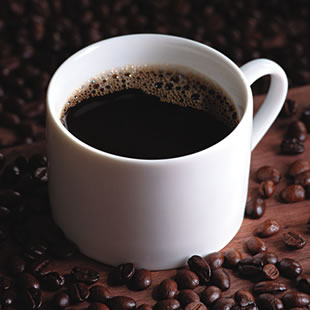
\includegraphics[width=\linewidth]{2-textuais/figs/coffee.jpg}
		\caption{Coffee.}
	\end{subfigure}
	\begin{subfigure}[b]{0.4\linewidth}
		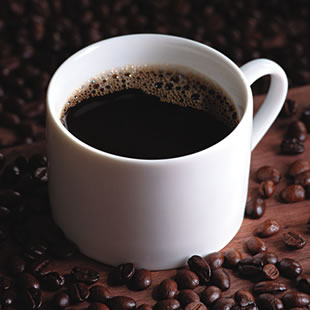
\includegraphics[width=\linewidth]{2-textuais/figs/coffee.jpg}
		\caption{More coffee.}
	\end{subfigure}
	\label{fig:coffee1}
	\legend{Fonte: Autor.}
\end{figure}


\begin{figure}[ht!]
	\centering
	\caption{The same cup of coffee. Two times.}
	\begin{subfigure}[b]{0.4\linewidth}
		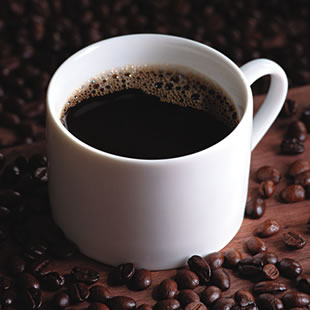
\includegraphics[width=\linewidth]{2-textuais/figs/coffee.jpg}
		\caption{Coffee.}
	\end{subfigure}
	\begin{subfigure}[b]{0.4\linewidth}
		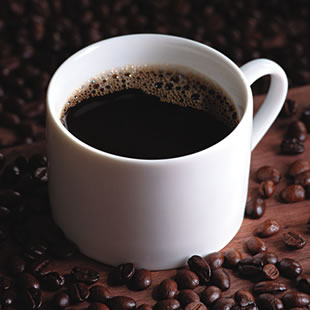
\includegraphics[width=\linewidth]{2-textuais/figs/coffee.jpg}
		\caption{More coffee.}
	\end{subfigure}
	\label{fig:coffee22}
	\legend{Fonte: Autor.}
\end{figure}
    
\begin{figure}[ht!]
	\centering
	\caption{The same cup of coffee. Again.}
	\begin{subfigure}[b]{0.2\linewidth}
		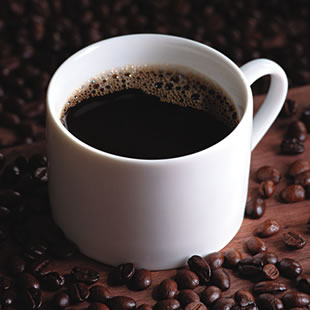
\includegraphics[width=\linewidth]{2-textuais/figs/coffee.jpg}
		\caption{Tasty coffee.}
	\end{subfigure}
    \begin{subfigure}[b]{0.6\linewidth}
		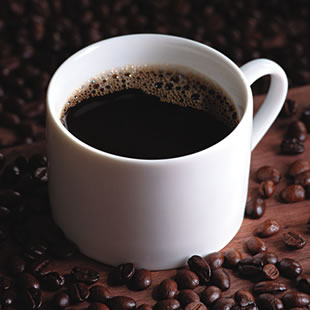
\includegraphics[width=\linewidth]{2-textuais/figs/coffee.jpg}
		\caption{Too much coffee.}
	\end{subfigure}
	\label{fig:coffee2}
	\legend{Fonte: Autor.}
\end{figure}

\begin{figure}[ht!]
	\centering
	\caption{The same cup of coffee. Multiple times.}
	\begin{subfigure}[b]{0.2\linewidth}
		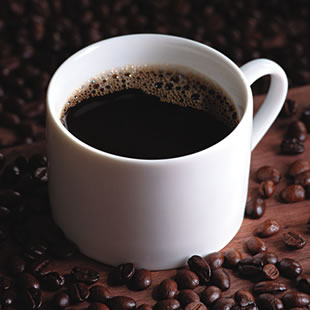
\includegraphics[width=\linewidth]{2-textuais/figs/coffee.jpg}
		\caption{Coffee.}
	\end{subfigure}
	\begin{subfigure}[b]{0.2\linewidth}
		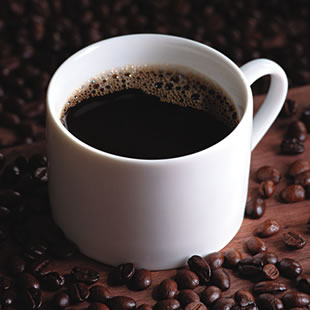
\includegraphics[width=\linewidth]{2-textuais/figs/coffee.jpg}
		\caption{More coffee.}
	\end{subfigure}
	\begin{subfigure}[b]{0.2\linewidth}
		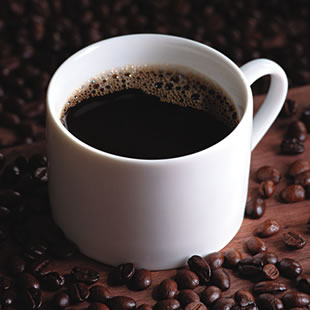
\includegraphics[width=\linewidth]{2-textuais/figs/coffee.jpg}
		\caption{Tasty coffee.}
	\end{subfigure}
    \begin{subfigure}[b]{0.5\linewidth}
		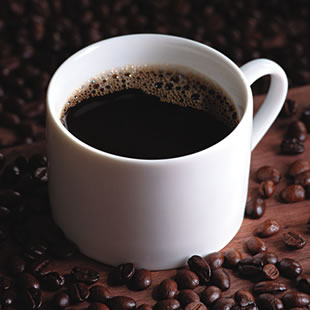
\includegraphics[width=\linewidth]{2-textuais/figs/coffee.jpg}
		\caption{Too much coffee.}
	\end{subfigure}
	\label{fig:coffee3}
	\legend{Fonte: Autor.}
\end{figure}

% ----------------------------------
% Resultados
\chapter{\bfseries Resultados}
\cite{santiago2014google}

% ----------------------------------------------------------
% Finaliza a parte no bookmark do PDF
% para que se inicie o bookmark na raiz
% e adiciona espaço de parte no Sumário
% ----------------------------------------------------------
\phantompart

% ----------------------------------
% Conclusão
\chapter{\bfseries  Conclusão}



% ----------------------------------
% Trabalhos Futuros
\chapter{\bfseries  Trabalhos Futuros}





\section{\bfseries Limitações}



% ----------------------------------------------------------
% ELEMENTOS PÓS-TEXTUAIS
% ----------------------------------------------------------
\postextual

% ---
% Referências
% ---
\bibliography{referencias-acervo}

% ---
% Glossário
% ---
%
% Consulte o manual da classe abntex2 para orientações sobre o glossário.
%
\glossary


% ---
% Apêndices
% ---
\begin{apendicesenv}
	\partapendices % Imprime uma página indicando o início dos apêndices
	%\addcontentsline{toc}{section}{Seção Não Numerada}
	%NBR 6029:2006: 3.3 apêndice: Texto ou documento elaborado pelo autor, a fim de complementar sua argumentação, sem prejuízo da unidade nuclear do trabalho. 

%----------------------------------------------------------
\chapter{\texorpdfstring{Nome Apêndice 1}{Nome Apêndice 1}}

% ----------------------------------------------------------

Texto ou documento elaborado pelo autor, a fim de complementar sua argumentação, sem prejuízo da unidade nuclear do trabalho. 

% ----------------------------------------------------------
\chapter{\texorpdfstring{Nome Apêndice 2}{Nome Apêndice 2}}
% ----------------------------------------------------------

Texto ou documento elaborado pelo autor, a fim de complementar sua argumentação, sem prejuízo da unidade nuclear do trabalho. 


%Comando para incluir um anexo-apendice arquivo em PDF:
%\includepdf[pages={-}]{3-pos-textuais/anexos/nomedoarquivo.pdf}


\end{apendicesenv}

% ---
% Anexos
% ---
\begin{anexosenv}
	\partanexos % Imprime uma página indicando o início dos anexos
	% NBR 14724:2011: 3.3: anexo:texto ou documento não elaborado pelo autor, que serve de fundamentação, comprovação e ilustração

% ---
\chapter{Nome anexo 1}
% ---

Um anexo é um documento que não foi elaborado pelo autor, ou seja, o autor apenas anexa. Anexos podem ser tabelas, mapas, diagramas, \textit{datasheets}, manuais e etc. 


% ---
\chapter{Nome anexo 2}
% ---

Um anexo é um documento que não foi elaborado pelo autor, ou seja, o autor apenas anexa. Anexos podem ser tabelas, mapas, diagramas, \textit{datasheets}, manuais e etc. 

% ---
\chapter{Nome anexo 3}
% ---

O autor pode anexar um PDF, traduzido como formato portátil de documento. 

Pode-se fazer uma descrição sucinta do arquivo anexado.

%Comando para incluir um anexo-apendice arquivo em PDF:
%\includepdf[pages={-}]{3-pos-textuais/anexos/nomedoarquivo.pdf}
	
\end{anexosenv}

% ---
% ÍNDICE REMISSIVO
% ---
\phantompart
\printindex

% Fim do documento ------------------------------------------
\end{document}